\documentclass[11pt]{report}
\usepackage[utf8]{inputenc}
\usepackage{epsfig}
\usepackage{verbatim}
\usepackage{ulem}
\usepackage{lscape}
\usepackage{multicol}
\usepackage{graphics}
\usepackage{amssymb}
\usepackage{fancyhdr}
\usepackage{fancybox}
\usepackage[table]{xcolor}
\usepackage[T1]{fontenc}
\usepackage{caption}
\usepackage{subcaption}
\usepackage{hyperref}
\usepackage{url}
\usepackage{listings}

\usepackage[a4paper]{geometry}
\geometry{top=1.8in, bottom=1.8in, left=1.5in, right=1.5in}

\setlength{\parindent}{0in}
\setlength{\parskip}{3mm}

% http://www.elec.ucl.ac.be/logistique/informatique/Digests/TeX/1999/texhax.04
\setcounter{secnumdepth}{5}   % depth of section numbering
\setcounter{tocdepth}{5}      % depth of section showing in TOC

\newcommand{\textdesc}[1]{\textit{\textbf{#1}}} % font for \descitem
\newcommand{\descitem}[1]{\item \textdesc{#1}}

\title{A distributed, collaborative development project of a Policy Engine for use in buildings\\\scalebox{0.85}{Global Software Development}}
\author{Berntsen, R., \url{raber@itu.dk}\\Hansen, K., \url{kben@itu.dk}\\Kokholm, T., \url{tkok@itu.dk}\\Stanciulescu, S., \url{scas@itu.dk}\\Wainach, N., \url{nicl@itu.dk}}

\begin{document}

\maketitle
\begin{abstract}

background, however, ...
what we	did (the innovative aspects)
contributions (design, evaluation) method
results / what it means

\end{abstract}
\tableofcontents

%%%%%%%%%%%%%%%%%%%%%%%%%%%%%%%%%%%%%%%%%%%%%%%%%%%%%%%%%%%%%%%%%%%%%%%%%%%%%%%%%%%%%%%%%%%%%%%%%%%%%%%%%%%%%%%%%%%%%%%%
%%%%%%%%%%%%%%%%%%%%%%%%%%%%%%%%%%%%%%%%%%%%%%%%%%%%%%%%%%%%%%%%%%%%%%%%%%%%%%%%%%%%%%%%%%%%%%%%%%%%%%%%%%%%%%%%%%%%%%%%
%%%%%%%%%%%%%%%%%%%%%%%%%%%%%%%%%%%%%%%%%%%%%%%%%%%%%%%%%%%%%%%%%%%%%%%%%%%%%%%%%%%%%%%%%%%%%%%%%%%%%%%%%%%%%%%%%%%%%%%%

\chapter{Introduction}
Natural resources are a precious commodity. Constructing resource efficient buildings makes sense, both in a political and economical perspective. Modern buildings today might come equipped with a suite of sensors and actuators, opening up for a degree of customizable control. Our collective need is that buildings can adapt to the users and the sensor-perceived environment, either automatically or manually. This can be achieved by developing policies that controls the actuators. Policies can be based on semi-static data, like time and weekdays. However this can have unforeseen and unwanted consequences. For example, a policy governing lightning activated merely by a static time schedule, might entail problems for people attending a rarely occurring late-night party in the building. If the building’s event calendar is accessible to the policy engine, a conditional event-checking statement might ensure continuous lighting. However, in order to achieve a more fine grained control, sensory input is needed. We define the interaction of these policies, as a task residing in Facility Management (FM). 

Without policies centralized control of a building is highly complex and error prone task, and the building might not be managed in a resource efficient way. By employing a policy engine, with access to the building’s sensors and actuators, both the building owner, the users and the administrators of the building benefits from the automation provided. If policies are correctly defined, building owners save energy and natural resources while providing extra comfort to their tenants. Building users can experience a building autonomously adjusting its internal environment to suit their comfort and needs. FM can achieve fine-grained control of the building, at a reduced workload. 
\newpage
In this paper we will; 1) document the collaborative project between the IT University of Copenhagen, Denmark and Strathmore University, Nairobi Kenya. 2) distill requirements from course provided material and a non-exhaustive literature search on policy engines, and 3) develop a software solution that implements these requirements.

Since this project was defined in the course Global Software Development at ITU, we have been provided a Building Simulator, making it up for a real building. The development focus of this project is therefore geared towards this simulator, and not for design and implementation challenges in doing a policy engine for a real building. The end product is a software based management console, that allow for centralized control of sensors and actuators in a building - by implementing a policy engine that allows for automated actuator responses based on sensor feedback, for example closing the blinds in excess sunlight or turning of the heater when windows are open.
\section{Context}

\section{Problem}

\chapter{Related Work}

\chapter{Method}

GSD: group organization, roles, meeting structure
Energy Efficient Building design approach
Virtual teams and distributed collaboration

\chapter{Design}

high level design
argument for it, discuss the alternatives
overall system architecture
components, relationships
limitations of your design

\begin{figure}[t]
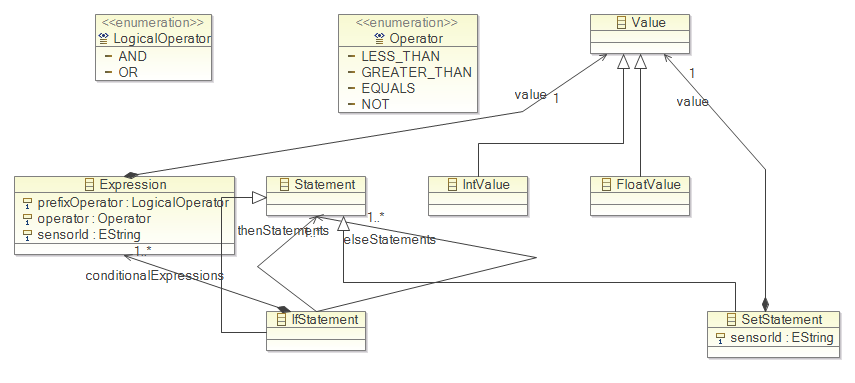
\includegraphics[width=1.00\columnwidth]{model.png}
\caption{Model}
\end{figure}

\chapter{Implementation}

\section{System}

\subsection{Interface Component}

\subsection{Abstraction Component}

\subsection{Storage Component}

\subsection{Request Flow}

\section{Collaboration Structure}

\subsection{Communication Protocol}


\chapter{Evaluation}

%%%%%%%%%%%%%%%%%%%%%%%%%%%%%%%%%%%%%%%%%%%%%%%%%%%%%%%%%%%%%%%%%%%%%%%%%%%%%%%%%%%%%%%%%%%%%%%%%%%%%%%%%%%%%%%%%%%%%%%%
%%%%%%%%%%%%%%%%%%%%%%%%%%%%%%%%%%%%%%%%%%%%%%%%%%%%%%%%%%%%%%%%%%%%%%%%%%%%%%%%%%%%%%%%%%%%%%%%%%%%%%%%%%%%%%%%%%%%%%%%
%%%%%%%%%%%%%%%%%%%%%%%%%%%%%%%%%%%%%%%%%%%%%%%%%%%%%%%%%%%%%%%%%%%%%%%%%%%%%%%%%%%%%%%%%%%%%%%%%%%%%%%%%%%%%%%%%%%%%%%%

\chapter{Discussion}

%%%%%%%%%%%%%%%%%%%%%%%%%%%%%%%%%%%%%%%%%%%%%%%%%%%%%%%%%%%%%%%%%%%%%%%%%%%%%%%%%%%%%%%%%%%%%%%%%%%%%%%%%%%%%%%%%%%%%%%%
%%%%%%%%%%%%%%%%%%%%%%%%%%%%%%%%%%%%%%%%%%%%%%%%%%%%%%%%%%%%%%%%%%%%%%%%%%%%%%%%%%%%%%%%%%%%%%%%%%%%%%%%%%%%%%%%%%%%%%%%
%%%%%%%%%%%%%%%%%%%%%%%%%%%%%%%%%%%%%%%%%%%%%%%%%%%%%%%%%%%%%%%%%%%%%%%%%%%%%%%%%%%%%%%%%%%%%%%%%%%%%%%%%%%%%%%%%%%%%%%%

\chapter{Conclusion}

%%%%%%%%%%%%%%%%%%%%%%%%%%%%%%%%%%%%%%%%%%%%%%%%%%%%%%%%%%%%%%%%%%%%%%%%%%%%%%%%%%%%%%%%%%%%%%%%%%%%%%%%%%%%%%%%%%%%%%%%
%%%%%%%%%%%%%%%%%%%%%%%%%%%%%%%%%%%%%%%%%%%%%%%%%%%%%%%%%%%%%%%%%%%%%%%%%%%%%%%%%%%%%%%%%%%%%%%%%%%%%%%%%%%%%%%%%%%%%%%%
%%%%%%%%%%%%%%%%%%%%%%%%%%%%%%%%%%%%%%%%%%%%%%%%%%%%%%%%%%%%%%%%%%%%%%%%%%%%%%%%%%%%%%%%%%%%%%%%%%%%%%%%%%%%%%%%%%%%%%%%

\bibliography{gsd}{}
\bibliographystyle{plain}
\addcontentsline{toc}{chapter}{References}

%%%%%%%%%%%%%%%%%%%%%%%%%%%%%%%%%%%%%%%%%%%%%%%%%%%%%%%%%%%%%%%%%%%%%%%%%%%%%%%%%%%%%%%%%%%%%%%%%%%%%%%%%%%%%%%%%%%%%%%%
%%%%%%%%%%%%%%%%%%%%%%%%%%%%%%%%%%%%%%%%%%%%%%%%%%%%%%%%%%%%%%%%%%%%%%%%%%%%%%%%%%%%%%%%%%%%%%%%%%%%%%%%%%%%%%%%%%%%%%%%
%%%%%%%%%%%%%%%%%%%%%%%%%%%%%%%%%%%%%%%%%%%%%%%%%%%%%%%%%%%%%%%%%%%%%%%%%%%%%%%%%%%%%%%%%%%%%%%%%%%%%%%%%%%%%%%%%%%%%%%%

\appendix

\chapter{Appendix}

\section{A.1. Requirements}

\section{A.2. Tests}

\end{document}

